\chapter{Local Correlation Methods (III): Excited State}

While local correlation methods for the ground state have been around since the 1980s, the extension of the local treatment of electron correlation to excited states is relatively new. With the earliest attempts dating back to the 2000s, many new approaches and approximations have emerged over the last decade, building on the concepts of LMOs, NOs and PNOs. One of the major obstacles that makes a straight-forward extension to excited states difficult is the long-range character of certain excitations, such as charge transfer states. In contrast to the description of electron correlation in the ground state, the occupied and virtual orbitals involved in electron transitions can be very far apart. This means that the optimal molecular orbital space for the excited state can be very different from that of the ground state. 

This chapter presents the state of the art for local correlated excited state methods (ADC, CCLR, EOM-CC) for LMOs, NOs, PNOs, and combinations thereof. Atomic orbital approaches are discussed as well. 

% Bau2017 CornFlex https://aip.scitation.org/doi/pdf/10.1063/1.4984820

% Linear‐scaling self‐consistent field methods for large molecules
% https://aip.scitation.org/doi/pdf/10.1063/1.2961039

\section{Low-Scaling Correlated Excited State Methods}

All of the existing low-scaling implementations of ADC, CCLR and EOM use some form of local or compact molecular orbital representation, to varying degrees of success. As mentioned above, the major problem that these methods face is the non-locality of certain excited states such as charge transfer states, which can involve occupied and virtually orbitals which are localized on entirely different parts in the system. Clearly, truncating virtual orbitals spatially is no longer a valid option, and makes a straight-forward extension of LMO-methods difficult, because they cut out far-away contributions. Similar problems are encountered in NO formulations, as the excited state is often not properly described by the electronic ground state (pair-)densities and their associated (pair) natural representation. Over the years, various strategies have been proposed to adapt existing LMO and NO schemes to excited states as well. 

\subsection{Orbital Invariance of the Matrix Expressions}

Correlated excited state methods involve some form of symmetric or non-symmetric eigenvalue problem, which is generally solved using the Davidson procedure. The time-determining step is given by the computation of the matrix-vector product of the ADC, response or EOM matrix with the Davidson trial vectors $\mbf{u}$
\begin{equation}
\mbf{r} = \mbf{A} \mbf{u}
\end{equation}
\noindent Closed expressions can be derived for the MVPs, with the matrix elements computed on the fly. The MVPs and trial vectors are divided into blocks of singles, doubles, triples, ... ($u_i^a$, $u_{ij}^{ab}$, $u_{ijk}^{abc}$) depending on the level of approximation of the underlying methods. In the case of ADC(2), the MVP is split according to
\begin{align}
r_{ia} &= A_{ia,jb} u_{jb} + A_{ia,jbkc} u_{jbkc} \\
r_{iajb} &= A_{iajb,kc} u_{kc} + A_{iajb,kcld} u_{kcld} 
\end{align}
\noindent The eigenvalue problem is generally solved in the canonical molecular orbital basis, but other orbital representations can also be used, by swapping all the CMO quantities $\cn{ia}{jb}$, $t_{iajb}$, ... by their local counterparts $\cn{\uli\ola}{\ulj\olb}$, $t_{\uli\ola\ulj\olb}, ...$. The eigenvalue problem can then be solved e.g. in an LMO basis, or the MVPs can be computed in the LMO basis and transformed to the CMO basis using the transformation matrix $\mbf{U}$:
\begin{equation}
r_{ia} = U_{i\uli} r_{\uli\ola} U_{\ola a} 
\end{equation}
\noindent The eigenvalues of the LMO matrix appear to not differ from the ones obtained via a CMO formalism \cite{Kats2009}.

For local EOM-CC and CCLR, the singles and doubles amplitudes $t_{\mu_1}$ and $t_{\mu_2}$ are determined iteratively from a local ground state calculations using the techniques in the previous chapter for reduced scaling. For the approximate EOM-CC2 and CC2-LR methods, as well as ADC(2), the MP2 amplitudes may also be computed iteratively in the local basis using the Hylleraas functional, or using a closed form expression via the Laplace transform techniques.   

EOM-CC2, CC2-LR and ADC(2) also allow an on-the-fly computation of the doubles part (see section \ref{sec:ADC_DAV}). Here, the orbital invariant formulation becomes less straight-forward because the doubles-doubles block of the non-canonical ADC and CC2 Jacobian matrix is not diagonal. Fortunately, the Laplace transform can be applied to circumvent this problem. Using the ADC(2) eigenvalue problem as an example, the doubles-folded MVP expression is given by
\begin{equation}
\begin{split}
r_{ia}(\omega) &= A_{ia,jb} u_{jb} + A_{ia,jbkc} \frac{A_{iajb,kc} u_{kc}}{\omega - \eps_a - \eps_b + \eps_i + \eps_j} \\
&= A_{ia,jb} u_{jb} - \sum_{\alpha}^{n} |w\pa| e^{\left(\omega - \eps_a - \eps_b + \eps_i + \eps_j\right) tpa} A_{ia,jbkc} A_{,kc} u_{kc} 
\end{split}
\end{equation}
After transforming to the LMO basis, the local ADC(2) equations read
\begin{equation}
r_{\uli \ola}(\omega) = A_{\uli \ola, \ulj \olb} u_{\ulj \olb} - A_{\uli \ola, \ulj \olb \ulk \olc} \sum_{\alpha}^{n} e^{\omega t\pa} X_{\ulj \ulj'}\pa Y_{\olb \olb'}\pa A_{\ulj' \olb' \ulk' \olc', \ull \old} u_{\ull \old} X_{\ulk \ulk'}\pa Y_{\olc \olc'}\pa  \\
\end{equation}
\noindent with the Laplace matrices $\mathbf{X}$ and $\mathbf{Y}$ 
\begin{equation}
X_{\uli\ulk}\pa = \sum_i U_{i\uli} |w^{'(\alpha)}|^{1/4} e^{\eps_i t^{'(\alpha)}} U_{k\ulk}
\end{equation}
\begin{equation}
Y_{\ola\olc}\pa = \sum_a U_{a\ola} |w^{'(\alpha)}|^{1/4} e^{-\eps_a t^{'(\alpha)}} U_{c\olc}
\end{equation}
\noindent Note that the optimal Laplace parameters $w^{'(\alpha)}$ and $t^{'(\alpha)}$ are different from the ones used in the MP2 amplitudes, due to the presence of the eigenvalue $omega$ in the denominator. Each time the eigenvalue changes, the Laplace parameters need to be recomputed to obtain an accurate approximation. 

An orbital invariant reformulation is not needed by every method. NOs, PNOs and NTOs can be \emph{canonicalized} (Annex \ref{app:CANON}) by diagonalizing the occupied-occupied and virtual-virtual block of the Fock matrix in the truncated NO/PNO/NTO basis to get a smaller set of canonical molecular orbitals and orbital energies. Because these types of representations generally do not depend on distance criteria, they are unaffected by the delocalized nature of the canonical basis, as they seek compactness rather than locality. 

\subsection{Local Molecular Orbitals and Domains}

The most challenging part in extending domain-specific virtual orbital methods to excited states lies in determining a suitable excitation domain in which to expand the virtual space. The first implementations of local excited state EOM-CCSD \cite{Kor2003,Cra2002} and CC2-LR \cite{Kat2003} constructed the domains using a Mulliken-charge like analysis of the CIS coefficients $r_ia$. The CIS coefficients are first transformed to the LMO-PAO basis
\begin{equation}
r_{\uli \olgm} = U_{\uli i } r_{ia} \bar{C}_{\mu a} 
\end{equation}
\noindent To determine the importance $w$ of each LMO/PAO, the squares of the norms of the coefficients are summed up row- and column-wise
\begin{equation}
\begin{split}
w_{\uli} &= \sum_{\mu} |r_{\uli \olgm}|^2 \\
w_{\olgm} &= \sum_{\uli} |r_{\uli \olgm}|^2
\end{split}
\end{equation}
\noindent The LMOs/PAOs are then ordered by decreasing weight. Their weights are then summed up until a certain threshold $T_{LMO}$/$T_{PAO}$ is reached (typically around 0.995 to 0.9999). The excited state orbital domains $[\uli]_{ES}$ containing the relevant virtual orbitals are then constructed by applying the Boughton-Pulay algorithm to a set of "excited natural orbitals" \cite{Kor2003}
\begin{equation}
\phi_{\uli}^* = \sum_{\ola} r_{\uli \olgm} \phi_{\olgm}  
\end{equation} 
\noindent The full orbital domain of $i$ is then given as the union of its ground-state and excited state domain $[\uli]$ = $[i]_{GS} \cup [i]_{ES}$. The virtual orbital weights $w_{\olgm}$ can be used to impose further restrictions on the virtual orbital space. Finally, the pair domains $ij$ are formed as the union $[\uli] \cup [\ulj]$. In general, only the computation of the doubles part, which is time-determining, is subject to domain-restrictions, while the singles part is computed without domain lists.

The method however has the major flaw that the orbital domains are highly sensitive to the CIS transition density, which does not describe the excited state very accurately. Some orbitals can be dropped in the domain construction which might become important for doubles contributions. LMO methods face an interesting chicken-or-egg problem where they need information from the excited state wave function, to accurately compute properties of said function. There are several ways to address this problem. In their local CC2-LR implementation, Kats and Schütz \cite{Kat2009} use Laplace transformed doubles folding to recompute the doubles amplitudes on the fly, which allows to adapt the excited state domains dynamically during the optimization procedure. Starting from the CIS transition density, the domains are recomputed at each step by analyzing the state vector $r_{\uli \olgm}(\omega)$ as described above. This greatly increased accuracy compared to canonical calculations with energy differences well below 0.1 eV.

Mester et al. \cite{Mes2017} proposed a more pragmatic approach, where they first analyze the CIS state vector to extract the important LMOs and PAOs. They then augment the domains $[i]_{EX}$ by adding all remaining molecular orbitals that have a significant Mulliken charge on an atom that is also significant for $i$. This is based on the assumption that, although CIS might not be a good approximation, the important orbitals should still be close by. 

Nonetheless, the LMO method is again plagued by spurious distance dependent thresholds and Mulliken charge thresholds. Nowadays, low scaling excited state methods are mostly dominated by PNOs, NOs, or NTOs.

% Kor2003 First EOM-CCSD Korona, T.; Werner, H.-J. Local treatment of electronexcitations in the EOM-CCSD method.J. Chem. Phys.2003,118,3006.
% Also first EOM-CCSD Cra2002 Crawford, T. D.; King, R. A. Locally correlated equation-of-motion coupled cluster theory for the excited states of largemolecules.Chem. Phys. Lett.2002,366, 611.
% https://aip.scitation.org/doi/10.1063/1.3237134

\subsection{Natural Orbitals}

NO methods achieve performance by dropping virtual natural orbitals with low occupation numbers. The first implementations of EOM-CC and CCLR in the NO representation used natural orbitals obtained from the diagonalization of the ground state MP2 density matrix \cite{Lan2010}. A reasonable speed-up could be observed, although the excited state character was not taken into account. However, it was shown \cite{Kum2017} that properties like the polarizability are much more sensitive to the truncation of the virtual orbitals than the ground state correlation energy, with the error increasing linearly as a function of the number of dropped virtual natural orbitals. While VNOs with low occupation numbers, i.e. diffuse character, can be safely  ignored for the ground state correlation energy, diffuse VNOs play a much more important role for response properties, and hence fewer VNOs can be omitted. Better results could be obtained by simply truncating the virtual CMOs instead, which invalidates the use of VNOs. 

In their NO-CC2 and NO-ADC(2) implementations, Mester et al. \cite{Mes2017, Mes2018, Mes2019} proposed to compute a set of occupied and virtual NOs by diagonalizing the occupied and virtual state-averaged densities
\begin{equation}
\mathbf{D}_{ij} = \frac{1}{2} \left( \mathbf{D}_{ij}^{MP2} + \mathbf{D}_{ij}^{CIS(D)} \right)
\end{equation}
\begin{equation}
\mathbf{D}_{ab} = \frac{1}{2} \left( \mathbf{D}_{ab}^{MP2} + \mathbf{D}_{ab}^{CIS(D)} \right)
\end{equation}
\noindent where $\mathbf{D}^{MP2}$ is the MP2 ground state density and $\mathbf{D}^{CIS}$ is the state-specific CIS(D) excited state density. Their restricted expressions read
\begin{equation}
D_{ij}^{MP2} = \sum_{kab} \left( 2 t_{ik}^{ab} t_{jk}^{ab} - t_{ik}^{ab} t_{jk}^{ab} \right) 
\end{equation}
\begin{equation}
D_{ab}^{MP2} = \sum_{ijc} \left( 2t_{ij}^{ca} t_{ij}^{cb} - t_{ij}^{ca}t_{ij}^{bc} \right)
\end{equation}
\begin{equation}
D_{ij}^{CIS(D)} = \sum_{a} c_i^a c_j^a  + \sum_{kab} \left( 2 t_{ik}^{ab} t_{jk}^{ab} - t_{ik}^{ab} t_{jk}^{ab} \right) 
\end{equation}
\begin{equation}
D_{ab}^{CIS(D)} = \sum_{i} c_i^a c_i^b + \sum_{ijc} \left( 2c_{ij}^{ca} c_{ij}^{cb} - c_{ij}^{ca}c_{ij}^{bc} \right)
\end{equation}
\noindent where $c_i^a$ are the CIS coefficients and the $c_{ij}^{ab}$ are the CIS(D) doubles coefficients
\begin{equation}
c_{ij}^{ab} = \frac{\sum_c \left[ \cn{ac}{bj} c_i^c + \cn{ac}{bi} c_j^c \right] - \sum_k \left[ \cn{kj}{ai} c_k^b + \cn{kj}{bj} c_k^a \right]}{D_{ij}^{ab} + \omega_{CIS}}
\end{equation}
\noindent The state-averaged density needs to be recomputed and diagonalized for each state because $\mathbf{D}^{CIS(D)}$ depends on the excitation energy $\omega$. While the CIS(D) density is much easier to compute than the ADC(2) or CC2-LR state density, it still scales with $\ccpx{5}$. To reduce the computational complexity, the density is constructed in a truncated orbital space: first, a set of occupied and virtual LMOs are chosen according to the CIS weighting criteria $w$ described in the previous section. The basis is augmented by spatially close orbitals, and then canonicalized to yield a highly compact orbital molecular space which lowers the cost of constructing the CIS(D) densities. 

In combination with natural auxiliary functions, this hybrid NO-LMO scheme can reduce the timings for CC2 and ADC(2) to such a drastic extent that the CIS pre-iterations become the time-determining step (Figure \ref{fig:MESTER}), with an additional error of only 2-4 meV. The reduced scaling however comes at a high prefactor when computing multiple different excitation energies. 

\begin{figure}
\centering
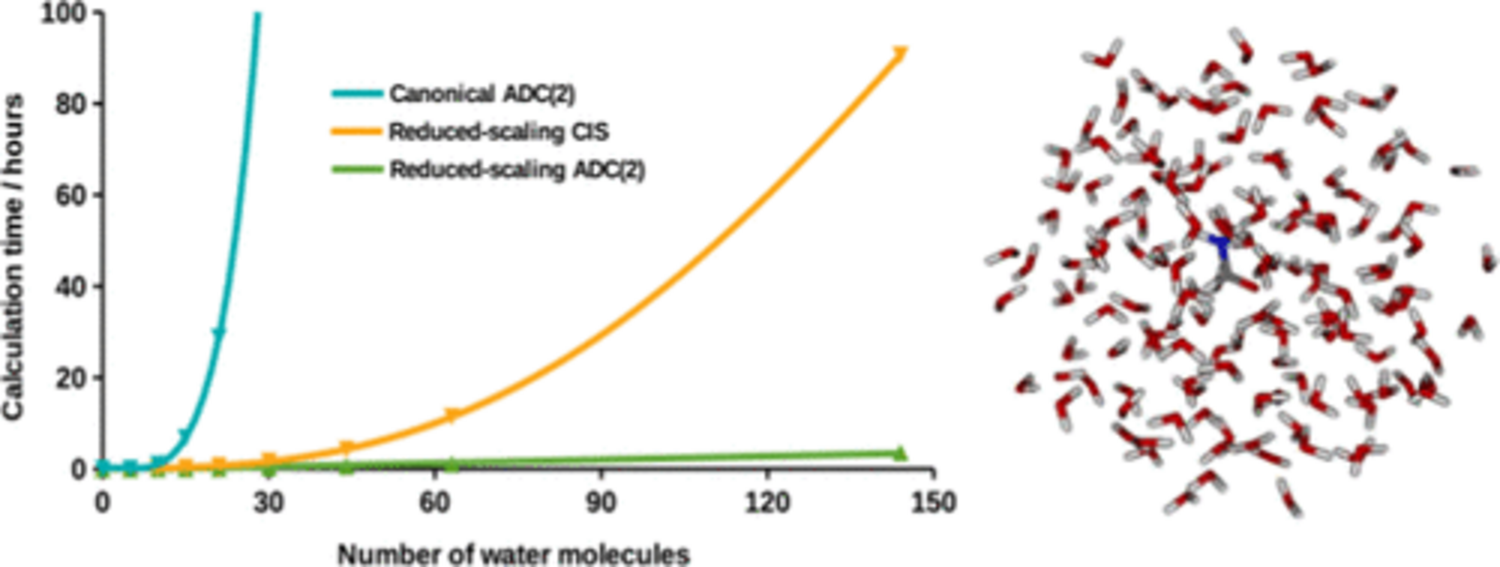
\includegraphics[scale=1.0]{Pics/mester_adc.png}
\caption{Wall times of CIS compared to NO-ADC(2) as a function of system size of hydrated formamide. Taken from \cite{Mes2019}.}
\label{fig:MESTER}
\end{figure}

% Reduced NO CC2 Mes2017 https://aip.scitation.org/doi/10.1063/1.4983277
% EOM NO Lan2010 https://aip.scitation.org/doi/10.1063/1.3276630
% CCLR NO Kum2017 https://pubs.acs.org/doi/10.1021/acs.jpca.6b11410
% Reduced ADC(2) Mes2018 https://aip.scitation.org/doi/10.1063/1.5021832
% Reduced ADC(2) Mes2019  https://pubs.acs.org/doi/pdf/10.1021/acs.jctc.9b00735
% CIS(D) Hea1994 https://www.sciencedirect.com/science/article/pii/0009261494000700?via%3Dihub

\subsection{Pair Natural Orbitals}

Pair natural orbital methods face the same problems as NOs, where PNOs with low occupation numbers are considerably more important for response properties than for ground state properties \cite{Har2016}. In a similar vein, excited state PNOs can be generated by considering lower level excited state electron pair densities \cite{Hel2011}. PNO methods have been successfully extended to ADC(2), CC2-LR \cite{Hel2013}, ADC(2)-x \cite{Hel2014} and CCSD-LR \cite{Fra2018} by using CIS(D) or CIS(D)-like densities
\begin{equation}
D_{ij}^{ab} = \sum_c \left( 2b_{ij}^{ab} - b_{ij}^{ba} \right) b_{ij}^{ab} + \left( 2b_{ij}^{ab} - b_{ij}^{ba} \right) b_{ij}^{ba}
\end{equation}
\noindent where $\mathbf{b}_{ij}$ are state-specific modified pair amplitudes which are not uniquely defined. Again, these methods come at the cost of a higher prefactor due to the relatively high cost of constructing PNOs. %Nonetheless, it was shown that the computational complexity can be lowered to $\ccpx{3}$ for PNO-CCSD-LR. 

Efforts have also been made to develop PNO response methods which are more economical for computing larger excitation manifolds by removing the state-specificity. Instead of taking individual excited state densities, Peng et al. \cite{Pen2018} proposed to generate a set of \emph{state-averaged} PNOs obtained by diagonalization of the average excited state density over an $N$-state manifold 
\begin{equation}
\mathbf{D}_{ij} = \frac{1}{N} \sum_k^N \mathbf{D}_{ij}^{(k)}
\end{equation}
\noindent A production-quality implementation has not yet been shown which uses this approach.

In their perturbed pair-natural orbital (PNO++) approach for CCLR, Cunha and Crawford \cite{Cun2021} incorporate the external perturbation into the electron pair density
\begin{equation}
D_{ij}^{ab} = \sum_c \left( 2x_{ij}^{ab} - x_{ij}^{ba} \right) x_{ij}^{ab} + \left( 2x_{ij}^{ab} - x_{ij}^{ba} \right) x_{ij}^{ba}
\end{equation}
\noindent where $\mathbf{x}$ are perturbed amplitudes given by
\begin{equation}
x_{ij}^{ab} = \frac{\overline{B}}{\ovl{H}_{aa} + \ovl{H}_{bb} - \ovl{H}_{ii} - \ovl{H}_{jj} + \omega}
\end{equation}
\noindent with an external perturbation $\ovl{B}$ and the similarity transformed Hamiltonian $\ovl{H}$. This gives a set of "perturbation-aware" PNOs customized for a given external perturbation \cite{Cra2019}. 

Finally, there are also the \emph{back-transformed} PNOs, or bt-PNOs, where the ground state PNO-quantities like the amplitudes are transformed back to the canonical basis and used in the canonical working equations \cite{Dut2016}.

In the end, most local excited state methods using natural orbitals differ by how they redefine the amplitudes $\mathbf{b}$ for the individual excited states or the whole perturbed molecular system. It is still an active field of research.

% PNO-CIS(D) Hel2011 https://aip.scitation.org/doi/10.1063/1.3664902 [Uses CIS(D) pair density]
% PNO-CC2 Hel2013 https://aip.scitation.org/doi/10.1063/1.4819071 [Uses Excited state OSVs to construct PNOs] 
% PNO-ADC(2)-x: Hel2014 https://www.sciencedirect.com/science/article/pii/S2210271X14001194?via%3Dihub [Also use excited state specific desnity to get OSVs using modified CIS(D) like desnities CC2/ADC(2)-x densities Dii_ab
% PNO-CCSD https://aip.scitation.org/doi/full/10.1063/1.5018514 [Also CIS(D) like density] 

% PNOs have similar Problem than NOs: Har2016  https://pubs.acs.org/doi/10.1021/acs.jctc.5b00898
% Because diffuseness. Solution: Cra2019 PNO++ https://onlinelibrary.wiley.com/doi/10.1002/wcms.1406
% PNO++-CCSD-LR Cun2021 https://pubs.acs.org/doi/pdf/10.1021/acs.jctc.0c01086

% State-averaged Pen2018 https://arxiv.org/pdf/1802.06738.pdf
% bt-PNOs Dut2016 https://aip.scitation.org/doi/pdf/10.1063/1.4958734
 
\subsection{Natural Transition Orbitals}

The last method to obtain a compact representation of excited states is via natural transition orbitals. NTOs are the equivalent of NOs for excited states, and represent a compact representations of their dominant contribution (Figure \ref{fig:NTO}). Baudin and Kristensen have developed two different CC2LR schemes based on NTOs called LoFEX (local framework for calculating excitation energies) \cite{Bau2016} and CornFLEX (correlated natural transition orbital framework for calculating excitation energies) \cite{Bau2017} 

Again, one needs information about the excited state to efficiently compute its properties. The LoFEX method starts with a time-dependent Hartree Fock calculation and generates a set of NTOs by decomposition of the TDHF transition vectors $\mathbf{r}$ by diagonalization
\begin{align}
\mathbf{r} \mathbf{r}^{\dagger} \mathbf{U} &= \lambda_o \mathbf{U} \\
\mathbf{r}^{\dagger} \mathbf{r} \mathbf{V} &= \lambda_v \mathbf{V}
\end{align}
\noindent which is just an alternative way to compute the occupied and virtual NTO transformation matrices $\mathbf{U}$ and $\mathbf{V}$, rather than by singular value decomposition. A set of dominant NTO pairs is then chosen for which their occupation numbers are above a given threshold $\tau_{LoFEX}$. The non-dominant NTOs are not discarded, but rather localized. The idea is to construct a surrounding excitation orbital space (XOS) containing LMOs that are important for correlation effects of the NTOs. A first guess to the XOS is chosen based on distance criteria and Löwdin charges. The CC2-LR eigenvalue problem is then solved in that basis, and new NTOs are computed from the CC2 transition vector and added to the XOS. This procedure is repeated until the excitation energy $\omega$ for that state has converged. While the guess XOS is first formed using distance criteria, the subsequent optimization procedure makes the method much more robust and black-box. Even for relatively small molecules, LoFEX can obtain considerable speed-ups. The main disadvantage is that LoFEX does not give any leverage for very delocalized excitations. 

The improved CornFLEX method constructs a set of CIS(D)-like NTOs (CIS(D')-NTOs) which is obtained from diagonalizing a CIS(D)-like density matrix in the CIS-NTO basis. As opposed to CIS-NTOs, the CIS(D') NTOs also include correlation effects and are a more robust representation that the simple ad-hoc extension of CIS-NTOs using LMOs. Speed-ups can be observed in CornFLEX even for delocalized excitations.

% Bau2016 https://aip.scitation.org/doi/pdf/10.1063/1.4953360
% Bau2017 https://aip.scitation.org/doi/pdf/10.1063/1.4984820

\begin{figure}
\centering
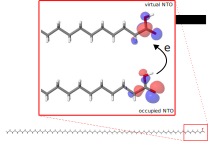
\includegraphics[scale=0.6]{Pics/NTOACID}
\caption{Dominant natural transition orbital pair for the lowest excitation of the carboxylic acid C$_{79}$H$_{159}$COOH ($\pi \rightarrow \pi^*$ transition). The span of the NTOs is very small compared to the rest of the molecule, and the compactness can be used to drastically speed up excited state calculations.}
\label{fig:NTO}
\end{figure}

\section{Atomic Orbital Configuration Interaction Singles}

%-> AO TDSCF (Kussmann)
%-> TDHF and RPA are equivalent in linear response regime. % see https://www.frontiersin.org/articles/10.3389/fphy.2019.00020/full

The methods presented in the previous section all work similarly. They first start by approximating the targeted excited states with a lower level of theory using CIS or CIS(D). They then solve higher order equations in the basis obtained from that approximation and may also dynamically augment the correlation domain while optimizing the excitation energies. The methods work on the principle of orbital \emph{compactness} rather than sparsity

At the moment of writing, CIS is the only excited state method which is routinely evaluated using an AO approach. While CIS does not give qualitatively good results, it is still a very important stepping stone for higher order methods, as was demonstrated in the previous section. Omitting the zero-order contributions, the CIS working equations are given by
\begin{equation}
u_{ia} = \left[ 2 \cn{ia}{jb} - \cn{ib}{ja} \right] u_{jb}
\end{equation}
\noindent Factoring out the MO coefficient matrices:
\begin{equation}
\begin{split}
u_{ia} &= C_{\mu i} C_{\sigma a} \left[ 2 \cn{\mu\sigma}{\nu\lambda} - \cn{\mu\lambda}{\nu\sigma} \right] C_{\nu j} C_{\lambda b} u_{jb} \\ 
&= C_{\mu i} C_{\sigma a} \left[ 2 \cn{\mu\sigma}{\nu\lambda} - \cn{\mu\lambda}{\nu\sigma} \right] P_{\nu\lambda} 
\end{split}
\end{equation} 
\noindent where $\mathbf{P}$ is the non-symmetric transition density in the AO basis. The CIS working equations can be reduced to the construction of a "pseudo"-Fock matrix which has a coulomb and an exchange part. The Fock matrix is then transformed to the MO basis:
\begin{align}
F_{\mu\nu} &= J_{\mu\nu} + K_{\mu\nu}  \\ 
u_{ia} &= C_{\mu i} F_{\mu\nu} C_{\mu a}  
\end{align}
\noindent For localized excitations, the AO transition density is sparse (Figure \ref{fig:CISDENSE}), and similar approximation can be used as in Hartree Fock, e.g. LinK, CFMM, or LDF. CIS can therefore be evaluated with $\mathcal{O}(N)$ computational effort. Strictly speaking, it is not a "pure" AO formulation, because the AO intermediates still need to be transformed to the MO basis.

\begin{figure}
\centering
\begin{subfigure}{0.3\linewidth}
\centering
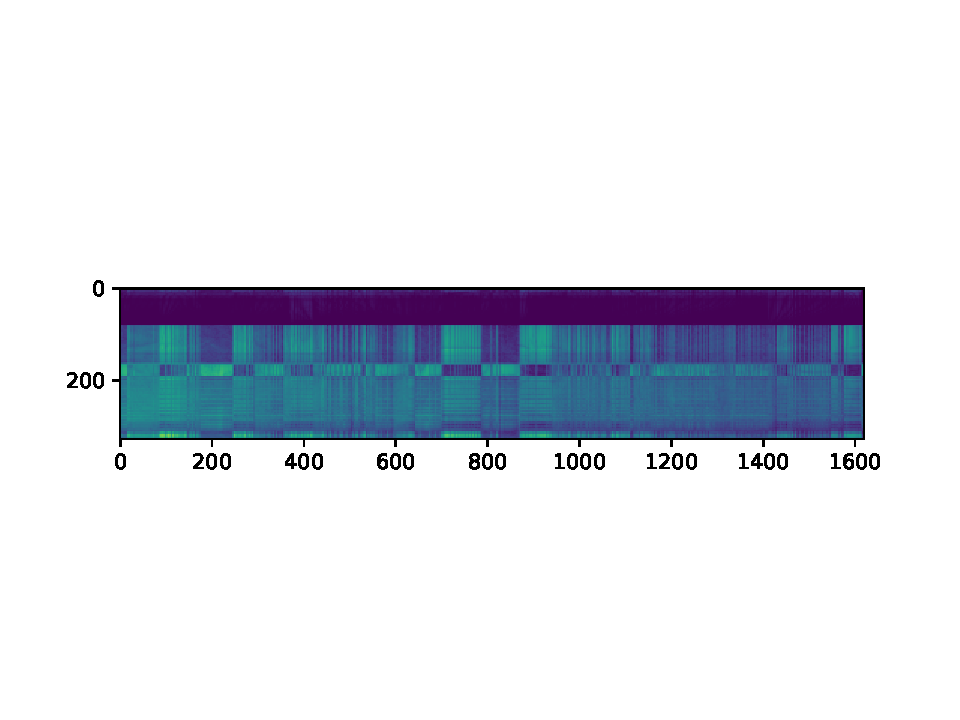
\includegraphics[scale=0.6]{Pics/CISDENSE}
\caption{}
\end{subfigure}
$\Longrightarrow$
\begin{subfigure}{0.6\linewidth}
\centering
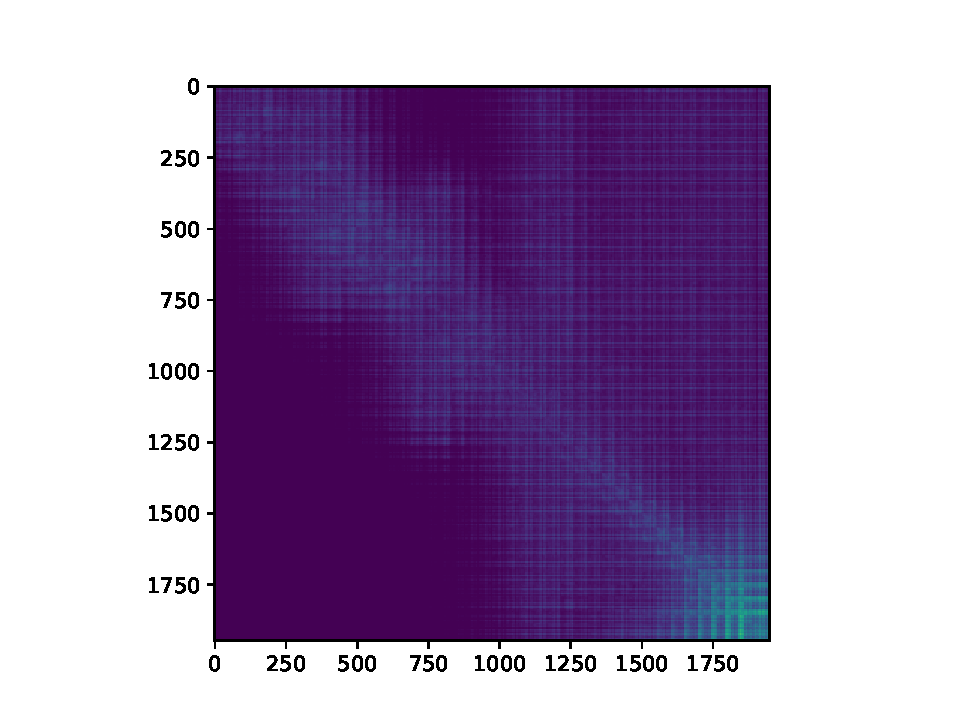
\includegraphics[scale=0.6]{Pics/CIS}
\caption{}
\end{subfigure}
\caption{Logarithm of the absolute values of the matrix elements in the transition densities in the MO (left) and AO basis (right) for the lowest excited state for the carboxylic acid C$_{79}$H$_{159}$COOH. The excitation domain is entirely localized on the carboxylic group. Using sparse matrix algebra, significant speed-ups can be obtained for CIS in the AO basis}
\label{fig:CISDENSE}
\end{figure}

% PAO CCLR not good! Look at Gunnar review article perhaps

% First appearance of local EOM-CCSD 
% Cra2002 https://aip.scitation.org/doi/pdf/10.1063/1.1537718

% First appearance of local CCLR CC2 (no doubles wrapping) Kat2006 https://aip.scitation.org/doi/pdf/10.1063/1.2339021
% Flaw: Domains dtermined from CCS, bad if not correponding to good approximat. ALso fixed during davidson

% Kat2009 https://aip.scitation.org/doi/pdf/10.1063/1.3237134
% FIxes Problem by refreshing domains

% state-specific PNOs from CIS(D) Hel2011 https://aip.scitation.org/doi/10.1063/1.3664902

% Hel2013 PNO-CC2 https://aip.scitation.org/doi/10.1063/1.4819071

% Hel2014 PNO-ADC2 https://www.sciencedirect.com/science/article/pii/S2210271X14001194?via%3Dihub

%PURE AO FORMULATION THOULESS INTEGRAL
%PROBLEM: MO ENERGIES ARE NEEDED. if a pure ao algorithm, most likely a whole other approach that tries to get "density metrix perturbation"

\section{Molecular Orbital-free Approaches}

Maybe if I have time
%https://aip.scitation.org/doi/full/10.1063/1.2961039?casa_token=XyapU_j1S9YAAAAA%3A6MKC3CuVoVEGS1bR-G3uHzyMo_UMcvArZKA2EkxO8Pwzc1gJWI0qwUWF6GB1PL7XEjDQH2lwrDniBQ
% https://aip.scitation.org/doi/10.1063/1.2965535